Considérons le dessin suivant, où les mesures des angles sont en radians.

\begin{center}
	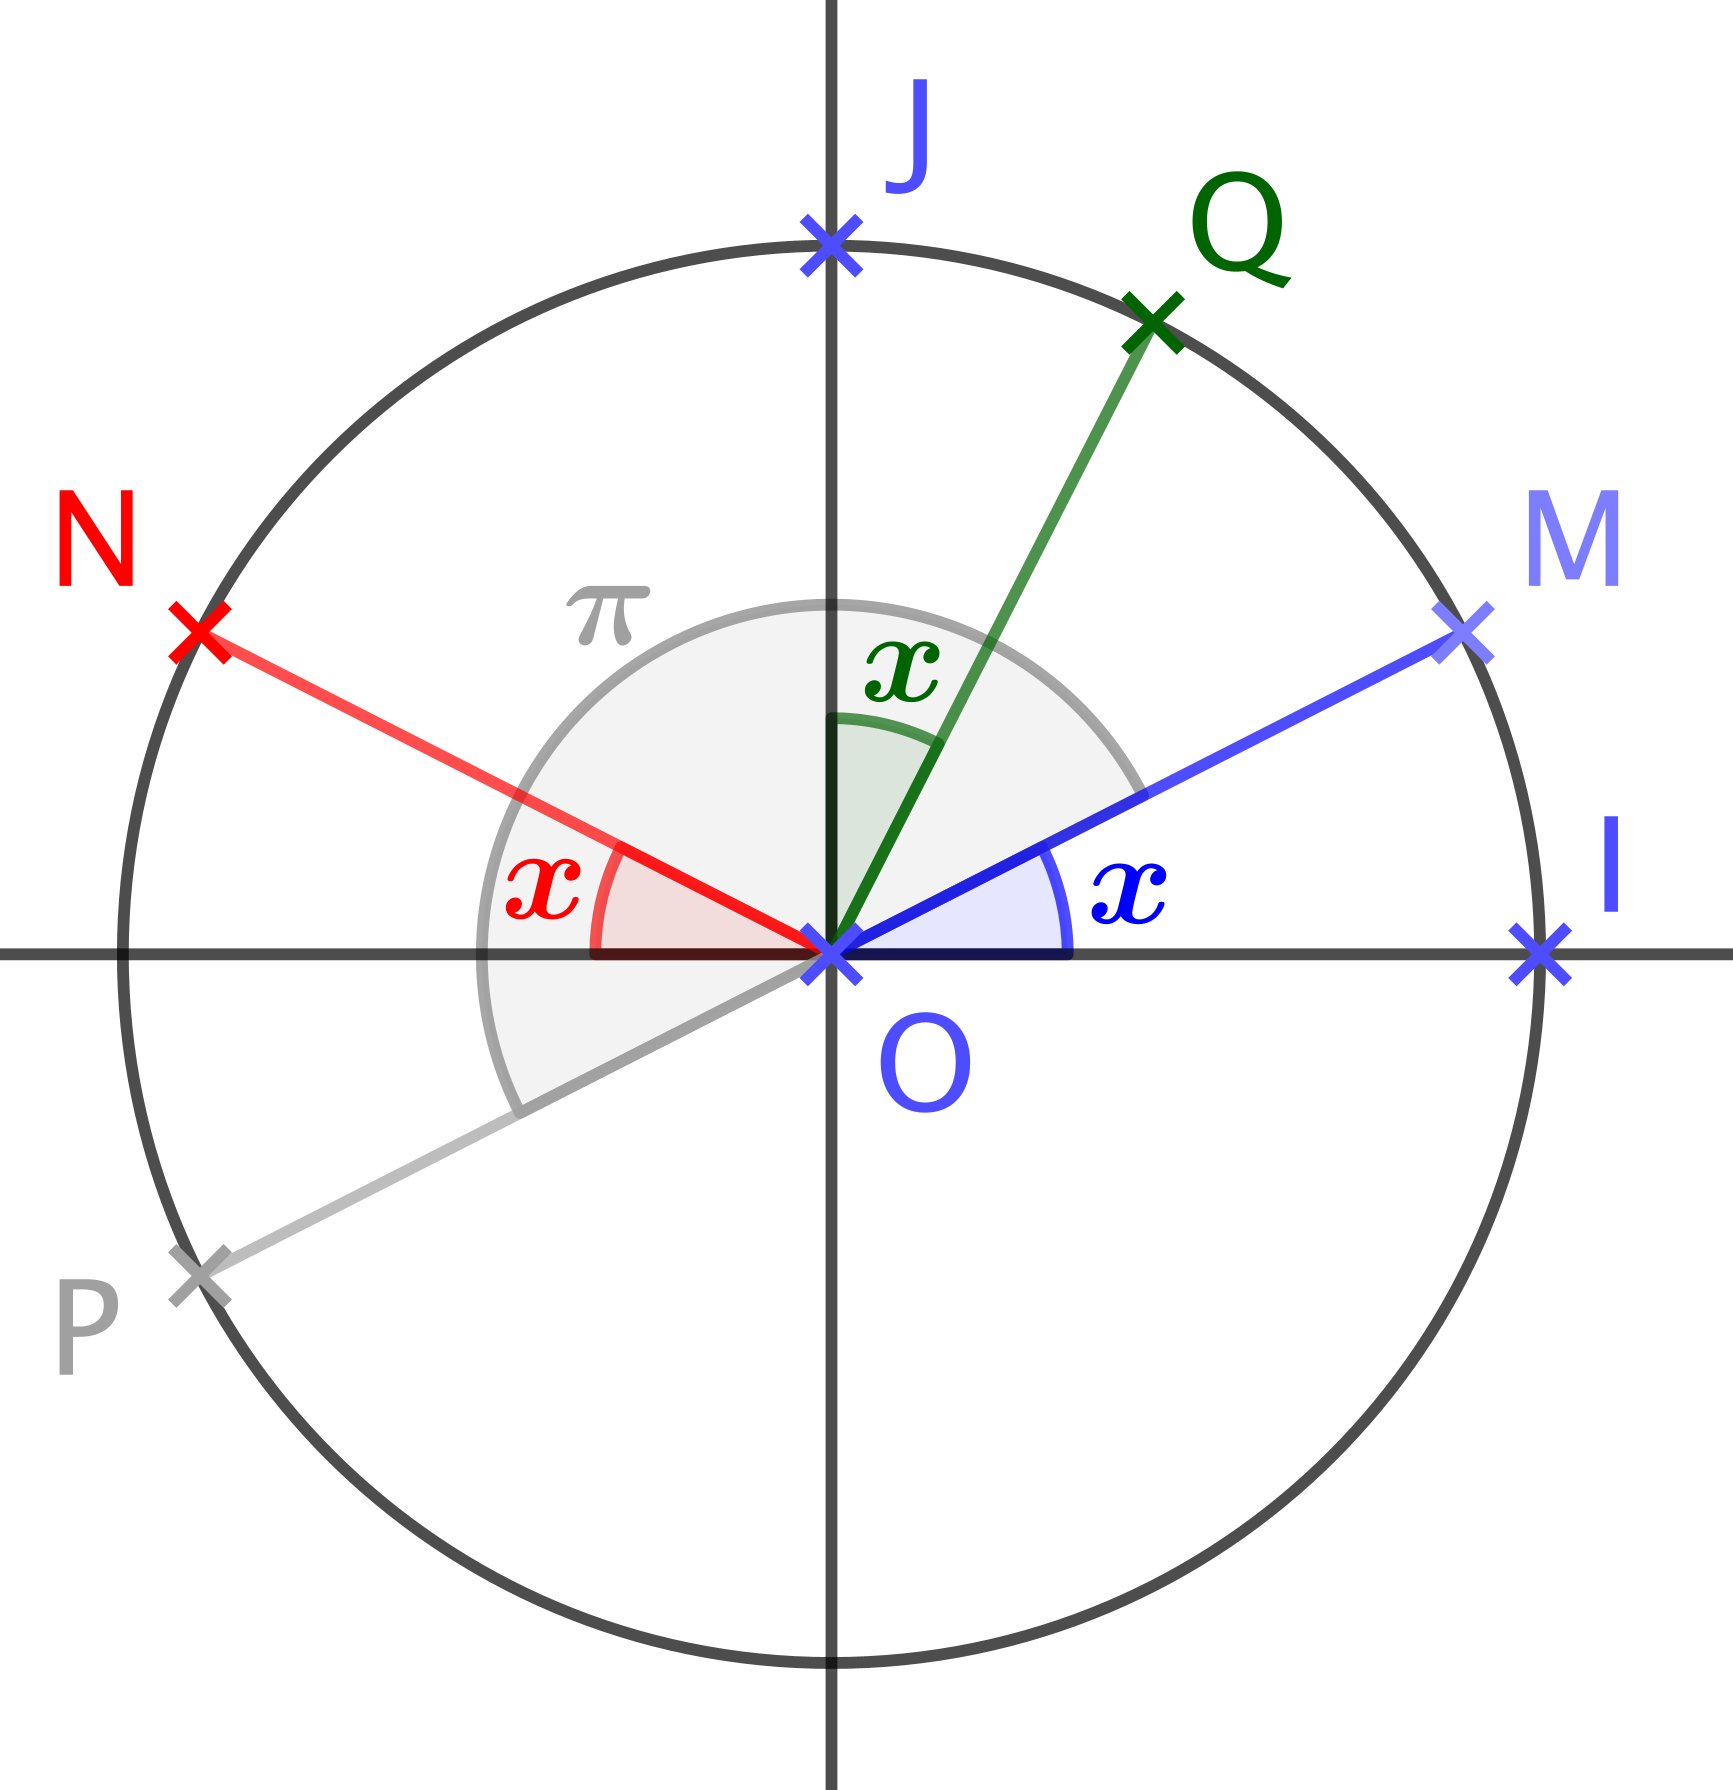
\includegraphics[scale = .7]{one-var-trig-formulas.png}
\end{center}

Via les points $M$, $N$, $P$ et $Q$, il est facile de fournir des arguments géométriques de symétrie justifiant que, sous la condition $x \in \intervalO{0}{\frac{\pi}{4}}$, nous avons:
%
\begin{multicols}{3}
\begin{itemize}[label=\small\textbullet]
	\item $\cos (\pi - x) = - \cos x$

	      \noindent
	      $\sin (\pi - x) = \sin x$ 

	\item $\cos (x + \pi) = - \cos x$

	      \noindent
	      $\sin (x + \pi) = - \sin x$

	\item $\cos \left( \frac{\pi}{2} - x \right) = \sin x$

	      \noindent
	      $\sin \left( \frac{\pi}{2} - x \right) = \cos x$ 
\end{itemize}
\end{multicols}


De nouveau, il serait bien de pouvoir passer, sans plus d'effort, à la validité des formules ci-dessus sur $\RR$ tout entier \emph{(considérer les autres cas n'est pas compliqué, mais c'est pénible)}.
%
Nous allons voir que cela est licite grâce au fait \ref{analytic-identity} suivant qui est un peu technique, car il nécessite la notion de fonction analytique.


\begin{defi}
    Soit $U \subseteq \RR$ un ouvert non vide.
	%
	Une fonction réelle $f: U \rightarrow \RR$ est dite analytique en $x_0$, 
	s'il existe
	une série entière $\dsum_{n = 0}^{+\infty} a_n x^n$
	de rayon de convergence $\rho_0 > 0$,
	et
	un réel $r \in \intervalOC{0}{\rho_0}$ tels que 
	$\forall x \in \intervalO{x_0 - r}{x_0 + r} \subseteq U$, on ait:
	$f(x) = \dsum_{n = 0}^{+\infty} a_n (x - x_0)^n$.

	Si $f$ est analytique en tout réel de $U$, nous dirons que $f$ est analytique sur $U$.
\end{defi}


\begin{fact} \label{analytic-identity}
    Soit $U \subseteq \RR$ un ouvert connexe non vide,
    et
    $f: U \rightarrow \RR$ une fonction analytique.
    %
	Si $f$ s'annule sur un ouvert de $U$, alors $f$ est identiquement nulle
	\emph{(c'est le théorème d'identité)}.  
\end{fact}


\begin{proof}
	Ceci découle du fait \ref{multi-analytic-identity} analogue pour plusieurs variables que nous démontrerons plus tard.
\end{proof}


\begin{fact} \label{power-series-vs-analytic}
    Soit $f: \RR \rightarrow \RR$.
    S'il existe une série entière $\dsum_{n = 0}^{+\infty} a_n x^n$ de rayon de convergence infini
    telle que
	$\forall x \in \RR$, $f(x) = \dsum_{n = 0}^{+\infty} a_n x^n$,
	alors
	$f$ est analytique sur $\RR$. 
\end{fact}


\begin{proof}
	Ceci découle du fait \ref{multi-power-series-vs-analytic} analogue pour plusieurs variables que nous démontrerons plus tard.
\end{proof}


Si nous revenons à nos identités trigonométriques, il suffit de savoir que les fonctions circulaires réelles sont analytiques sur $\RR$ tout entier, et de noter que le raisonnement géométrique au début de cette section fait clairement apparaître des zéros non isolés pour les fonctions analytiques sur $\RR$ suivantes.%
\footnote{
	Nous admettrons ces affirmations qui ne sont pas violentes à démontrer une fois que l'on a les bases de la théorie des fonctions analytiques.
}
%
\begin{itemize}[label=\small\textbullet]
	\item $f_1(z) = \cos (\pi - z) + \cos z$ 
	   et $f_2(z) = \sin (\pi - z) - \sin z$ 

	\smallskip
	\item $f_3(z) =\cos (z + \pi) + \cos z$ 
	   et $f_4(z) =\sin (z + \pi) + \sin z$

	\smallskip
	\item $f_5(z) =\cos \left( \frac{\pi}{2} - z \right) - \sin z$ 
	   et $f_6(z) =\sin \left( \frac{\pi}{2} - z \right) - \cos z$ 
\end{itemize}








\newpage


Que faire si nous avons des formules trigonométriques impliquant deux variables? Par exemple, le dessin suivant, par simple application des définitions géométriques du cosinus et du sinus, donne à la fois
$\cos(\alpha + \beta) = \cos \alpha \cos \beta - \sin \alpha \sin \beta$
et
$\sin(\alpha + \beta) = \cos \alpha \sin \beta + \sin \alpha \cos \beta$
pour
$(\alpha ; \beta) \in \big( \RRsp \big)^2$ tel que $0 < \alpha + \beta < \frac{\pi}{2}$. 

\begin{center}
	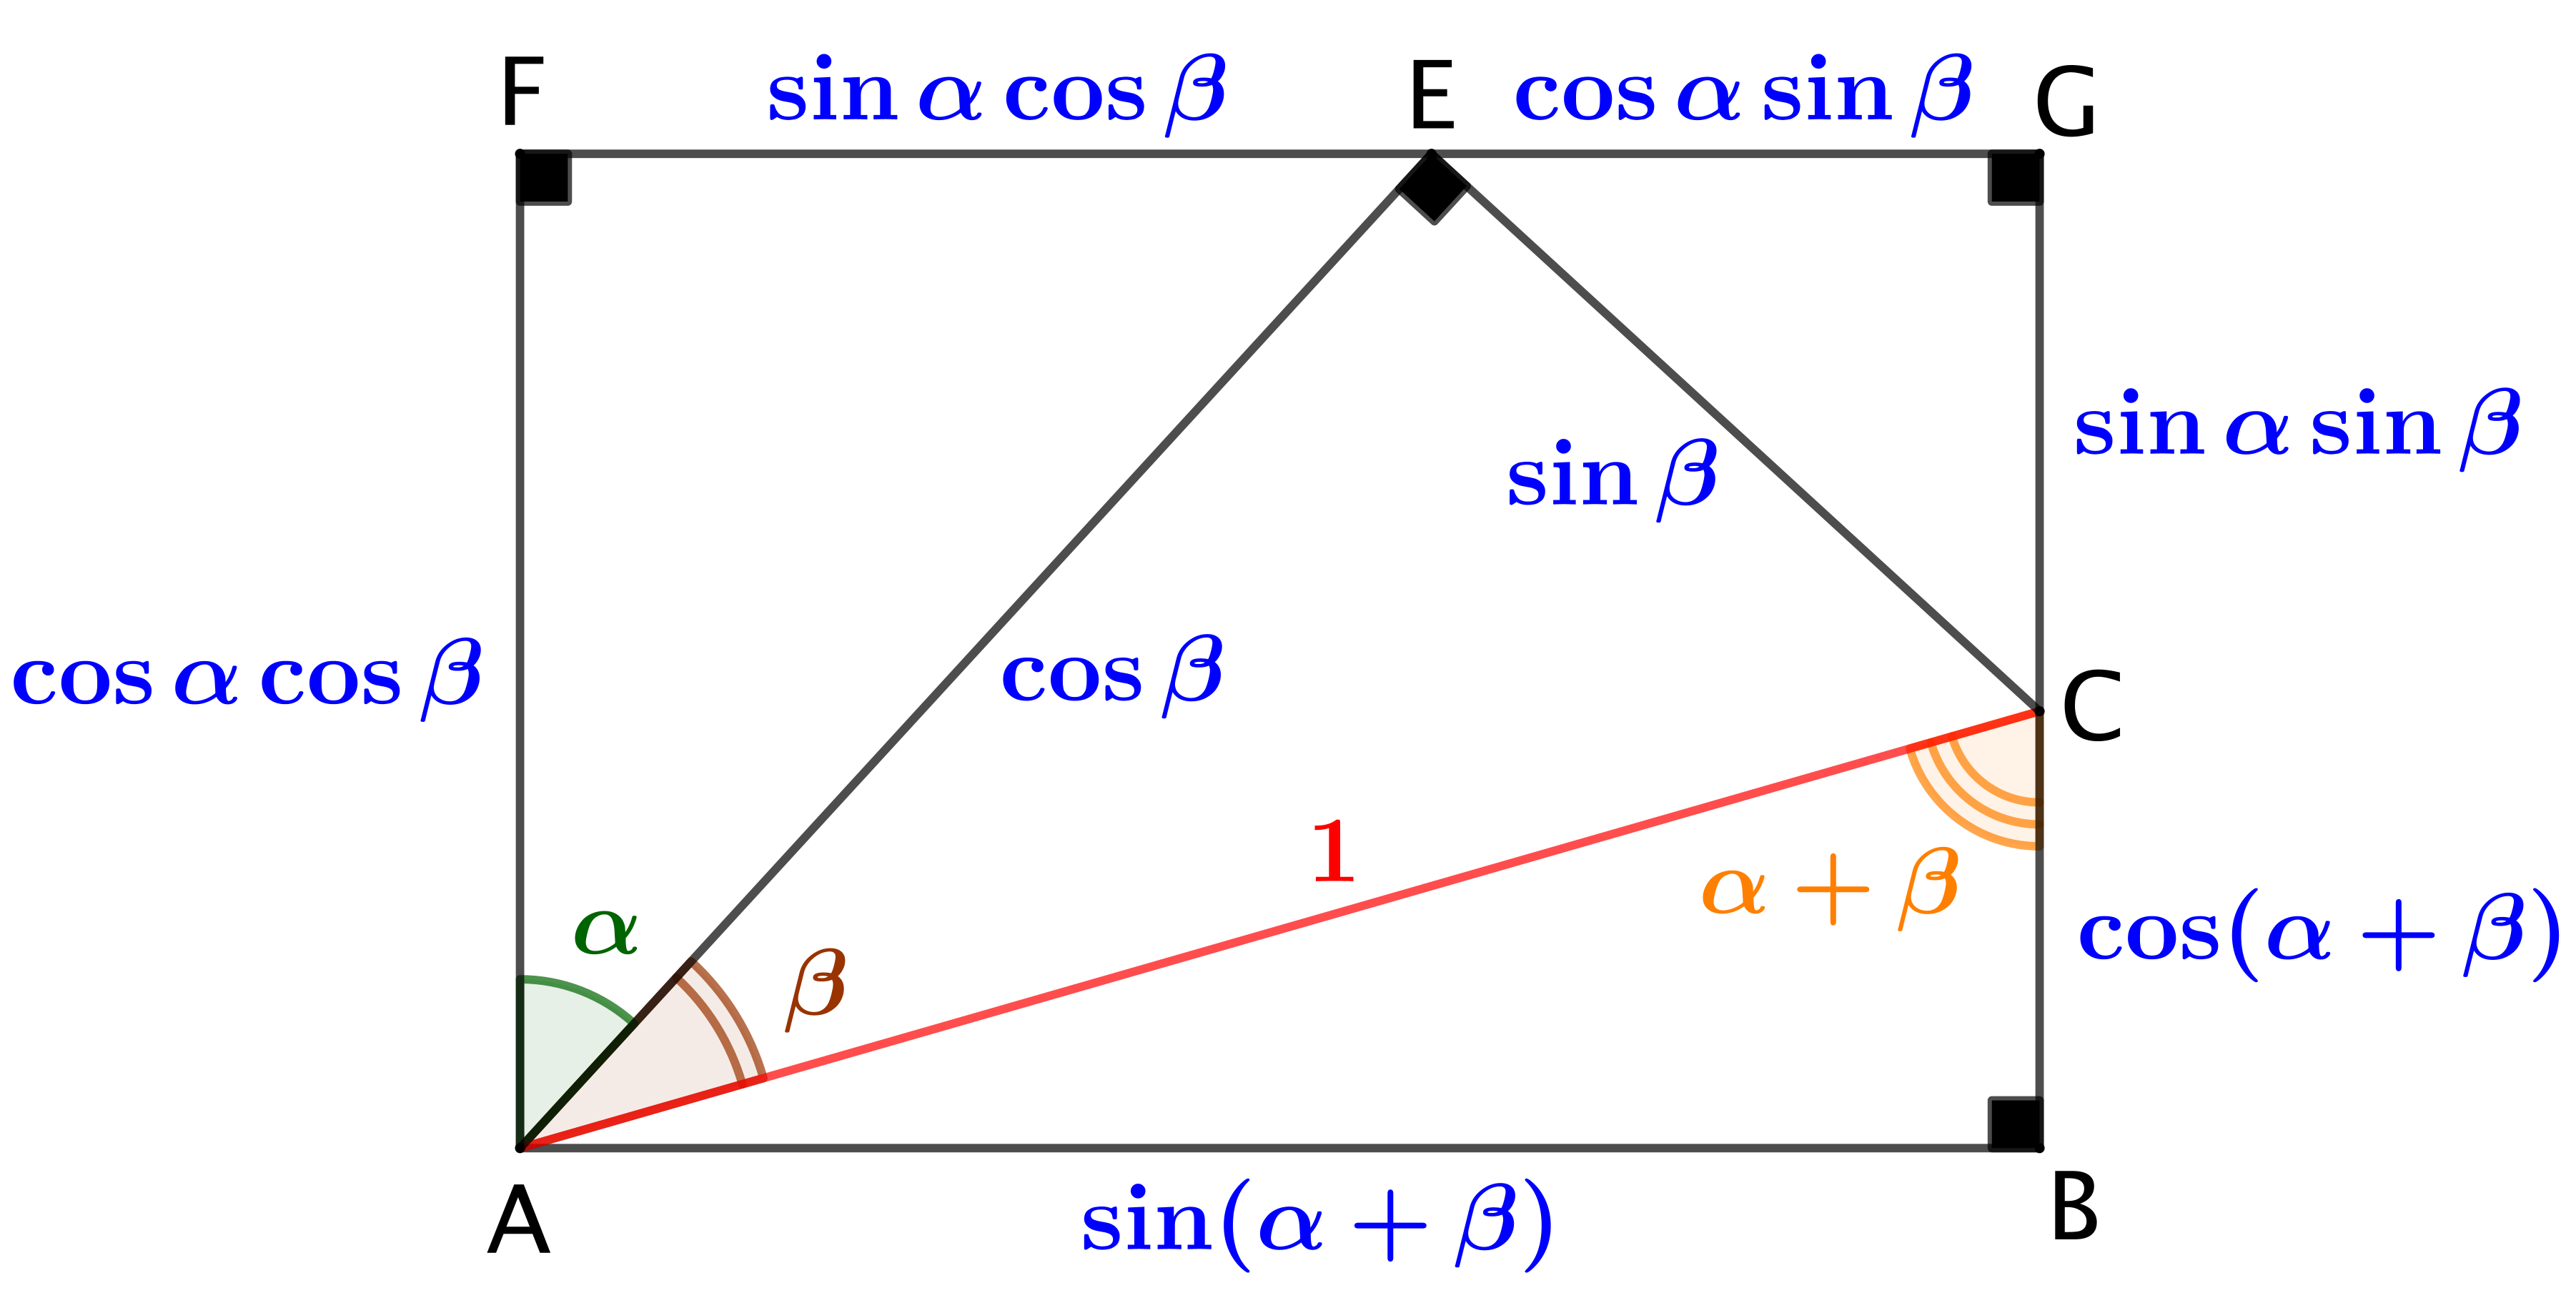
\includegraphics[scale=.7]{two-var-trig-formulas.png}
\end{center}

Le fait \ref{multi-analytic-identity} ci-dessous, qui généralise le fait \ref{analytic-identity}, implique la validité des formules trigonométriques précédentes sur $\RR^2$ tout entier en faisant les choix ci-après.
Nous voilà sauvés!
%
\begin{itemize}[label=\small\textbullet]
	\item $f_1(\alpha ; \beta) = \cos(\alpha + \beta) - \cos \alpha \cos \beta + \sin \alpha \sin \beta$

	\item $f_2(\alpha ; \beta) = \sin(\alpha + \beta) - \cos \alpha \sin \beta - \sin \alpha \cos \beta$
\end{itemize}






\begin{defi}
    Soient $n \in \NNs$, et $U \subseteq \RR$ un ouvert non vide.
	Une fonction réelle $f: U \rightarrow \RR$ est dite analytique en $x_0$, 
	s'il existe
	une série entière $\dsum_{n = 0}^{+\infty} a_n x^n$
	de rayon de convergence $\rho_0 > 0$,
	et
	un réel $r \in \intervalOC{0}{\rho_0}$ tels que 
	$\forall x \in \topodisc{x_0}{r} \subseteq U$, on ait:
	$f(x) = \dsum_{XXX} a_n (x - x_0)^n$.
	%
	Si $f$ est analytique en tout réel de $U$, on dira que $f$ est analytique sur $U$.
\end{defi}



\begin{fact} \label{multi-power-series-vs-analytic}
    Soient $n \in \NNs$, et $f: \RR^n \rightarrow \RR$.
    S'il existe une série entière $\dsum_{XXXX} a_n x^n$ de rayon de convergence infini
    telle que
	$\forall x \in \RR^n$, $f(x) = \dsum_{XXX} a_n x^n$,
	alors
	$f$ est analytique sur $\RR^n$. 
\end{fact}


\begin{proof}
	TODO
\end{proof}



\begin{fact} \label{multi-analytic-identity}
    Soient $n \in \NNs$, et $U \subseteq \RR^n$ un ouvert connexe non vide,
    et
    $f: U \rightarrow \RR$ une fonction analytique.
    %
	Si $f$ s'annule sur un ouvert de $U$, alors $f$ est identiquement nulle
	\emph{(c'est le théorème d'identité)}.  
\end{fact}


\begin{proof}
	TODO
\end{proof}